\section{Parte 1: Creación de una prueba y generación del código} 
\begin{itemize}
 \item  Cree un proyecto de biblioteca de clases .NET Standard en C char. Este proyecto contendrá el código
que quiere probar. Asigne al proyecto el nombre MyMath.
\begin{center}
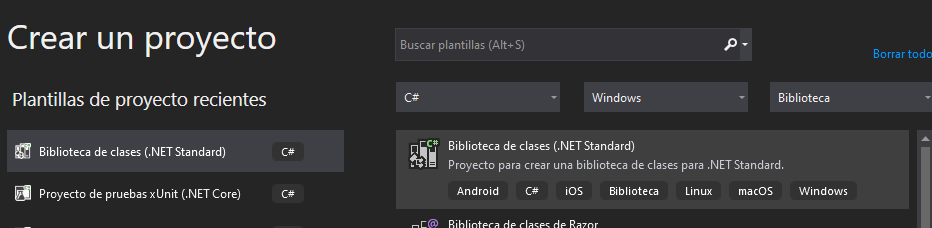
\includegraphics[width=\columnwidth]{images/1}\newline
\end{center}
 \item  En la misma solución, agregue un nuevo proyecto de prueba de MSTest (.NET Core) . Asigne al
proyecto de prueba el nombre MathTests.
 \item
\begin{center}
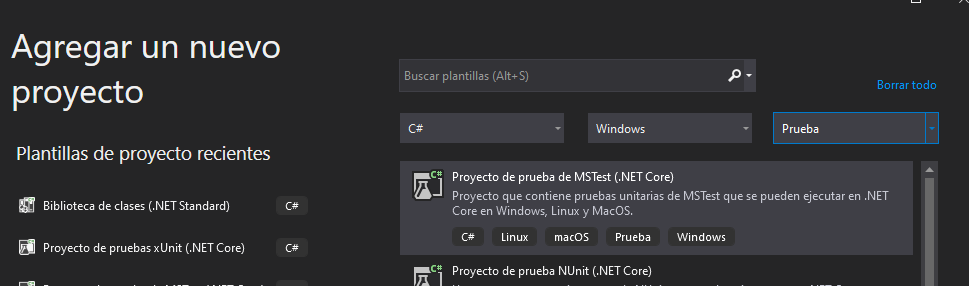
\includegraphics[width=\columnwidth]{images/2}\newline
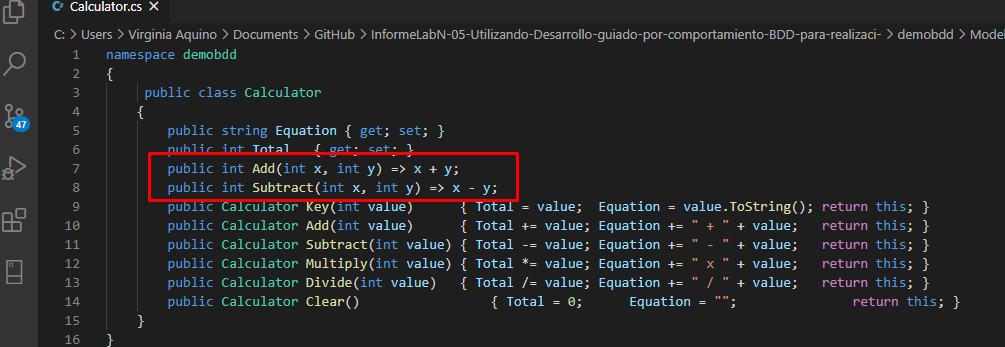
\includegraphics[width=\columnwidth]{images/001}\newline
\end{center} 
 \item Escriba un método de prueba simple que compruebe el resultado obtenido para una entrada
específica. Agregue el código siguiente a la clase UnitTest1:
\begin{center}
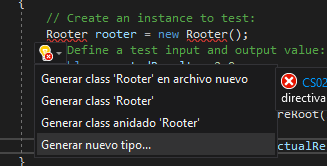
\includegraphics[width=\columnwidth]{images/3}\newline
\end{center} 
\item En el cuadro de diálogo Generar tipo, establezca Proyecto en MyMath, el proyecto de biblioteca
de clases y, luego, elija Aceptar.
\begin{center}
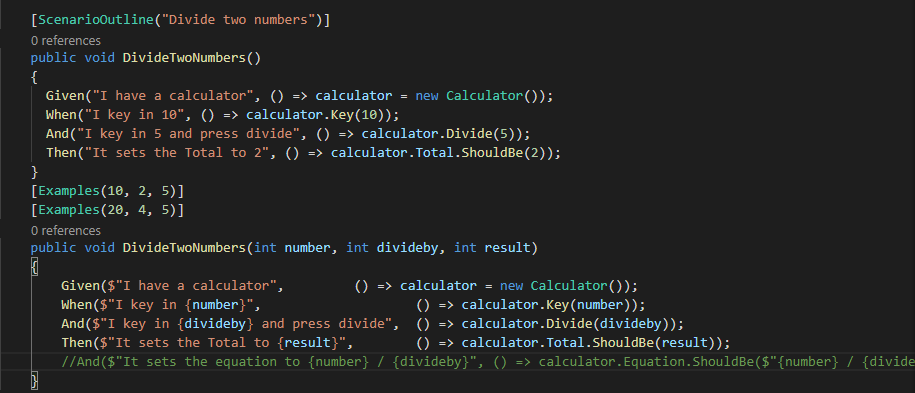
\includegraphics[width=\columnwidth]{images/4}\newline
\end{center} 
\item Genere un método a partir del código de prueba. Coloque el cursor en SquareRoot y, luego, en el menú
de bombilla, elija Generar método "Rooter.SquareRoot"
\begin{center}
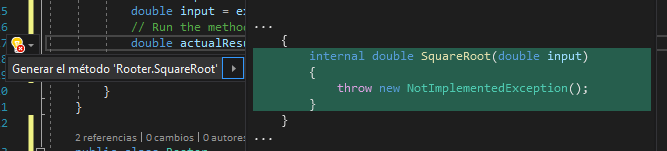
\includegraphics[width=\columnwidth]{images/5}\newline
\end{center} 
\item Ejecute la prueba unitaria
\begin{center}
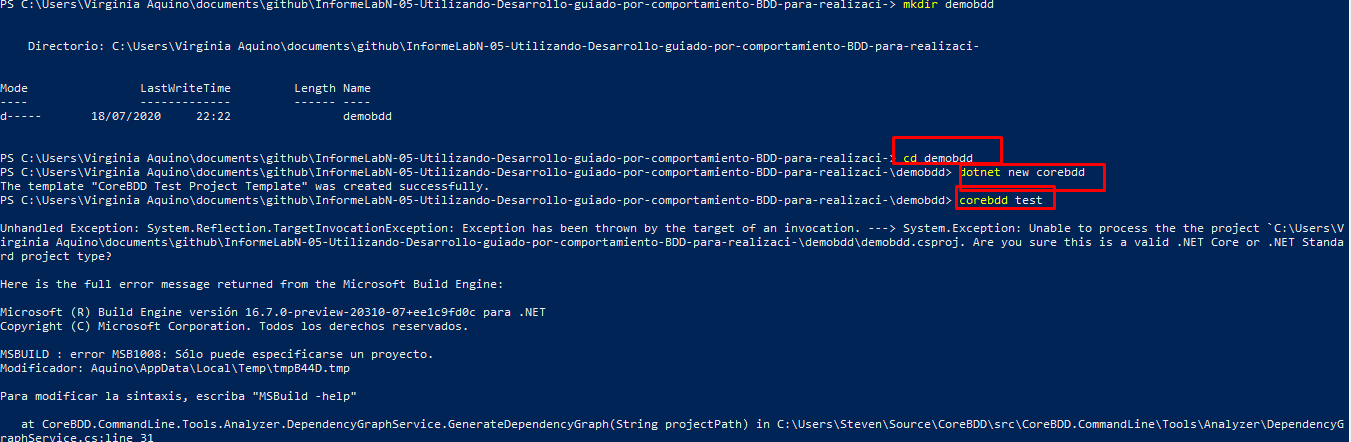
\includegraphics[width=\columnwidth]{images/6}\newline
\end{center} 
\end{itemize}
\section{Comprobación de un cambio en el código } 
\begin{itemize}
\item En el archivo Class1.cs, mejore el código de SquareRoot:
\begin{center}
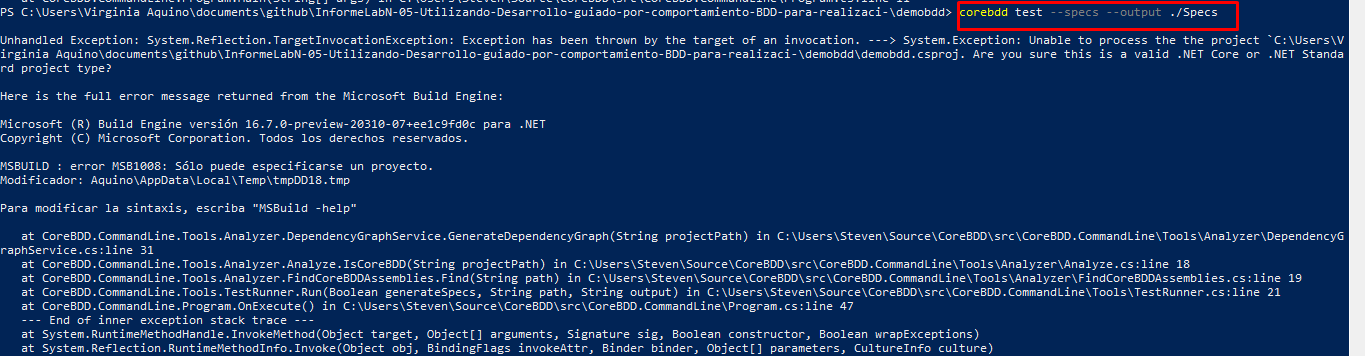
\includegraphics[width=\columnwidth]{images/7}\newline
\end{center}
\item En el Explorador de pruebas, elija Ejecutar todo.
\begin{center}
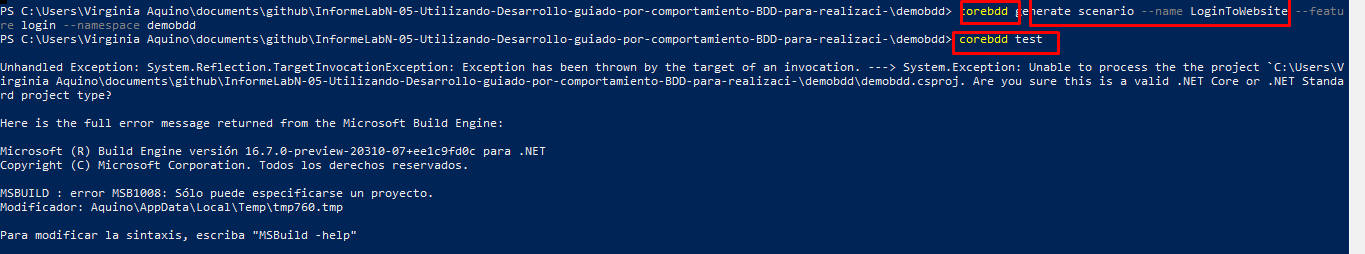
\includegraphics[width=\columnwidth]{images/8}\newline
\end{center}
\end{itemize}

\section{Extensión del intervalo de entradas} 

\begin{itemize}

\item En la clase de prueba, agregue la siguiente prueba para un intervalo de valores de entrada:
\begin{center}
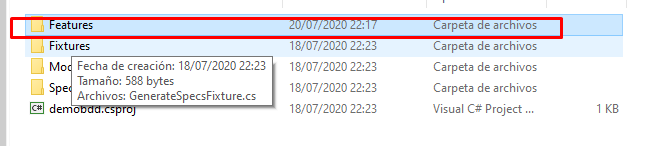
\includegraphics[width=\columnwidth]{images/10}\newline
\end{center}
\item En el Explorador de pruebas, elija Ejecutar todo.
\begin{center}
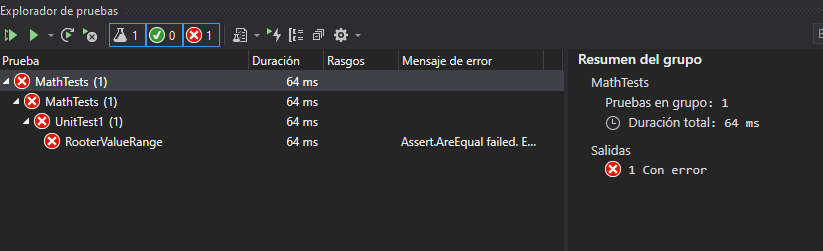
\includegraphics[width=\columnwidth]{images/11}\newline
\end{center}
\item Inspeccione el método que se está probando para ver qué puede ser incorrecto. Modifique el
código SquareRoot de la forma siguiente:
\begin{center}
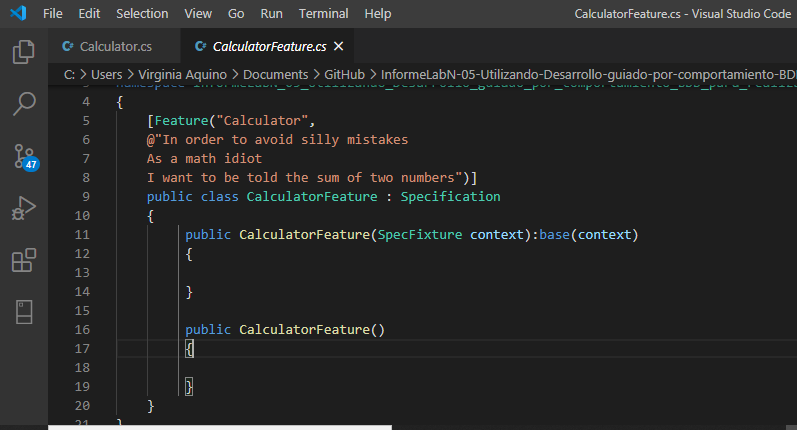
\includegraphics[width=\columnwidth]{images/002}\newline
\end{center}
\item En el Explorador de pruebas, elija Ejecutar todo.
\begin{center}
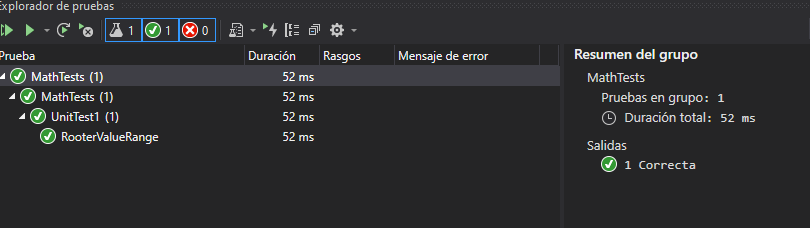
\includegraphics[width=\columnwidth]{images/12}\newline
\end{center}
\end{itemize}
\section{Agregue pruebas para casos excepcionales} 

\begin{itemize}

\item Agregue una nueva prueba para entradas negativas:
\begin{center}
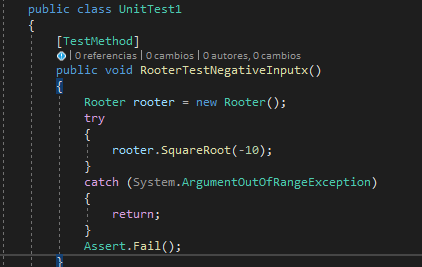
\includegraphics[width=\columnwidth]{images/13}\newline
\end{center}
\item En el Explorador de pruebas, elija Ejecutar todo.
\begin{center}
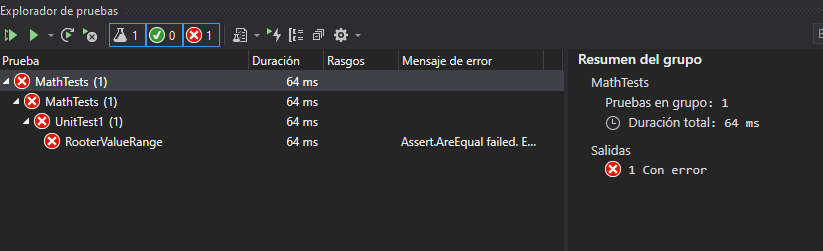
\includegraphics[width=\columnwidth]{images/11}\newline
\end{center}
\item Corrija el código SquareRoot; para ello, agregue la siguiente instrucción if al principio del método:
\begin{center}
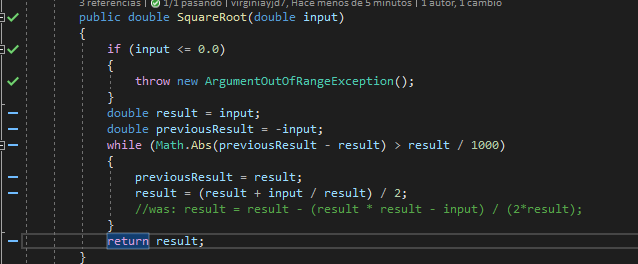
\includegraphics[width=\columnwidth]{images/16}\newline
\end{center} 
\item En el Explorador de pruebas, elija Ejecutar todo.
\begin{center}
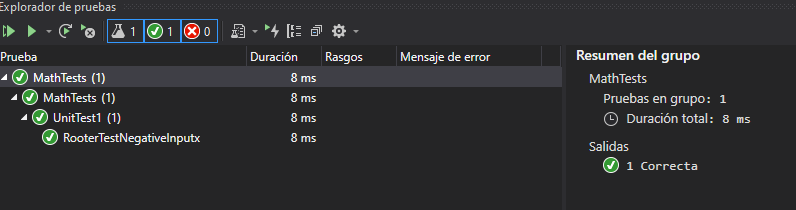
\includegraphics[width=\columnwidth]{images/17}\newline
\end{center} 
\end{itemize}

\section { Refactorizar el codigo en pruebas } 

\begin{itemize}

\item Cambie la línea que calcula result en el método SquareRoot de la manera siguiente:
\begin{center}
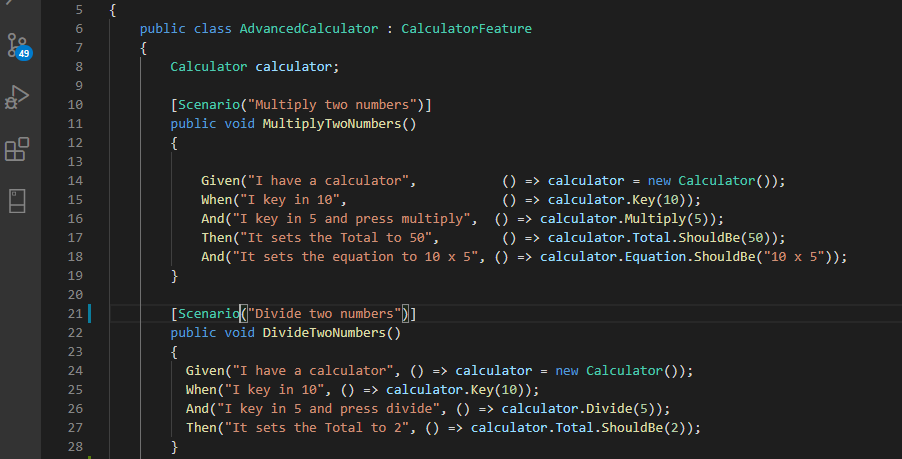
\includegraphics[width=\columnwidth]{images/004}\newline
\end{center} 
\item Elija Ejecutar todo y compruebe que todas las pruebas se siguen superando.
\begin{center}
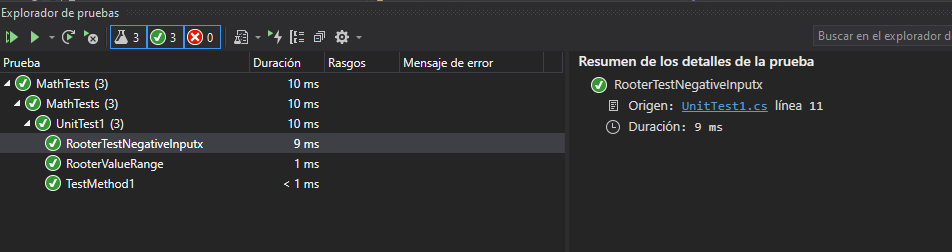
\includegraphics[width=\columnwidth]{images/005}\newline
\end{center}

\end{itemize}
\section{Parte 2: Creación de una prueba unitaria utilizando un framework de pruebas (XUnit) } 

\begin{itemize}

\item Ejecutamos los siguientes comandos:
\begin{center}
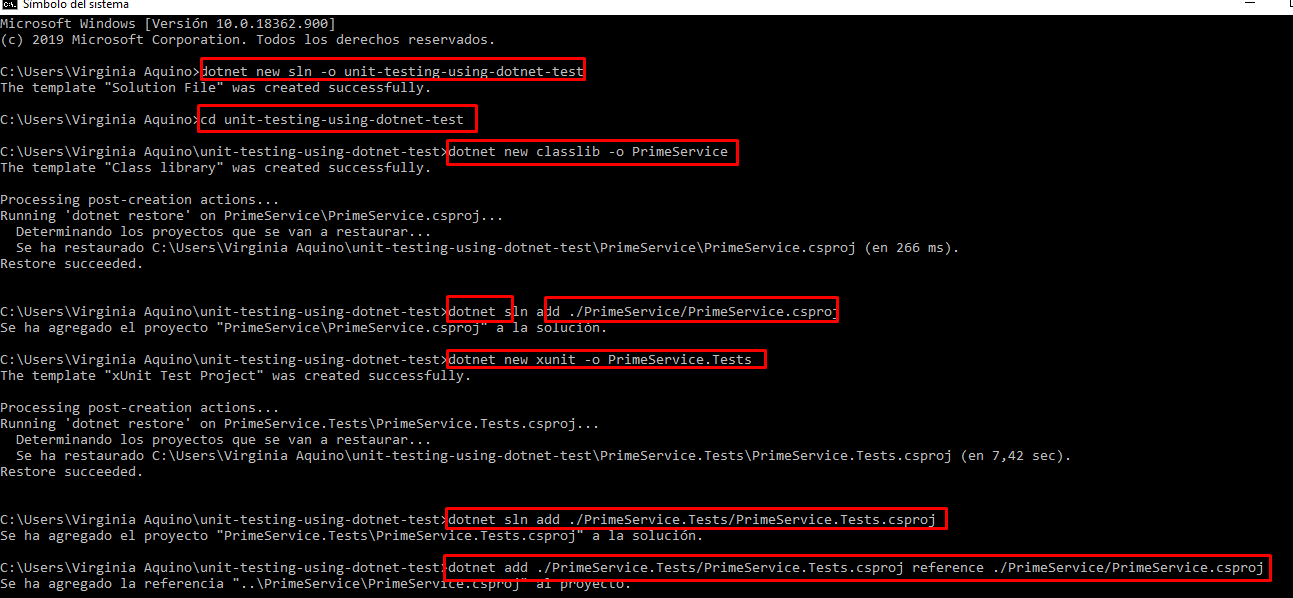
\includegraphics[width=\columnwidth]{images/lab2}\newline
\end{center} 

\end{itemize}
\section{Crea una prueba } 
\begin{itemize}

\item Actualice el proyecto PrimeService.Tests :

\begin{center}
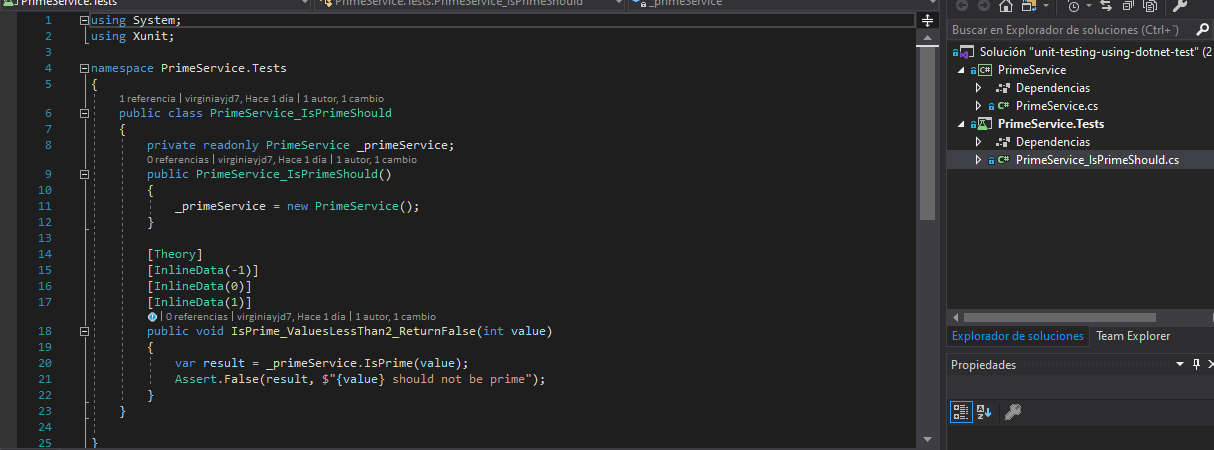
\includegraphics[width=\columnwidth]{images/lab3}\newline
\end{center} 
\item Ejecuta el corredor de prueba.La prueba falla porque IsPrimeno se ha implementado. Usando el enfoque TDD, escriba
solo el código suficiente para que esta prueba pase. Actualice IsPrimecon el siguiente
código:
\begin{center}
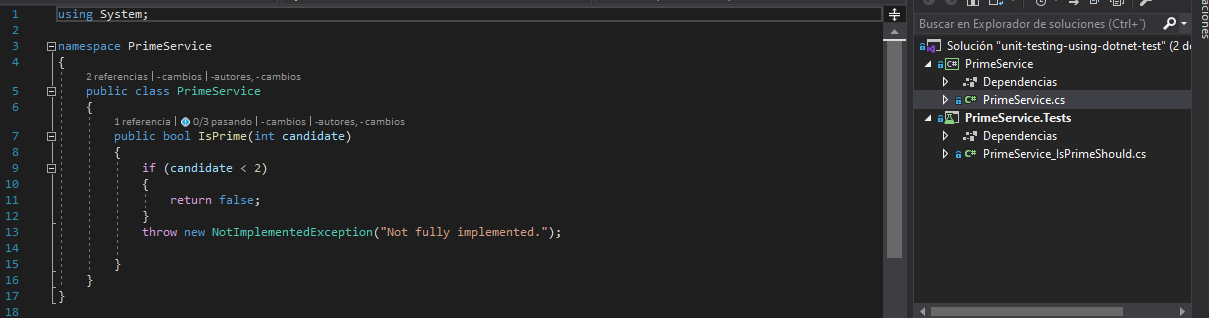
\includegraphics[width=\columnwidth]{images/lab4}\newline
\end{center} 
\item Ejecutar dotnet test. La prueba pasa.
\begin{center}
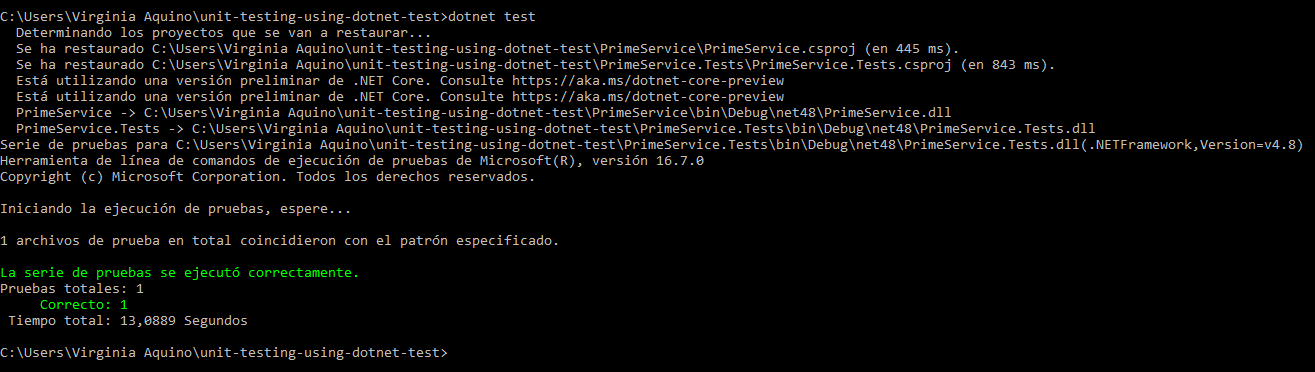
\includegraphics[width=\columnwidth]{images/resultado2}\newline
\end{center} 
\item Reemplace el siguiente código:
\begin{center}
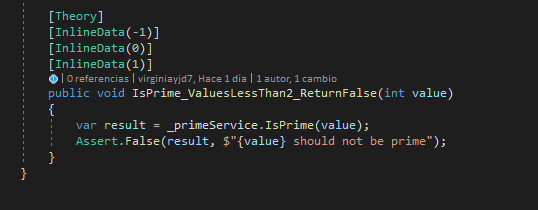
\includegraphics[width=\columnwidth]{images/lab5}\newline
\end{center} 
\item En el código anterior, [Theory]y [InlineData]habilite probar varios valores menores que
dos. Dos es el número primo más pequeño.Ejecutar dotnet test, dos de las pruebas fallan:
\begin{center}
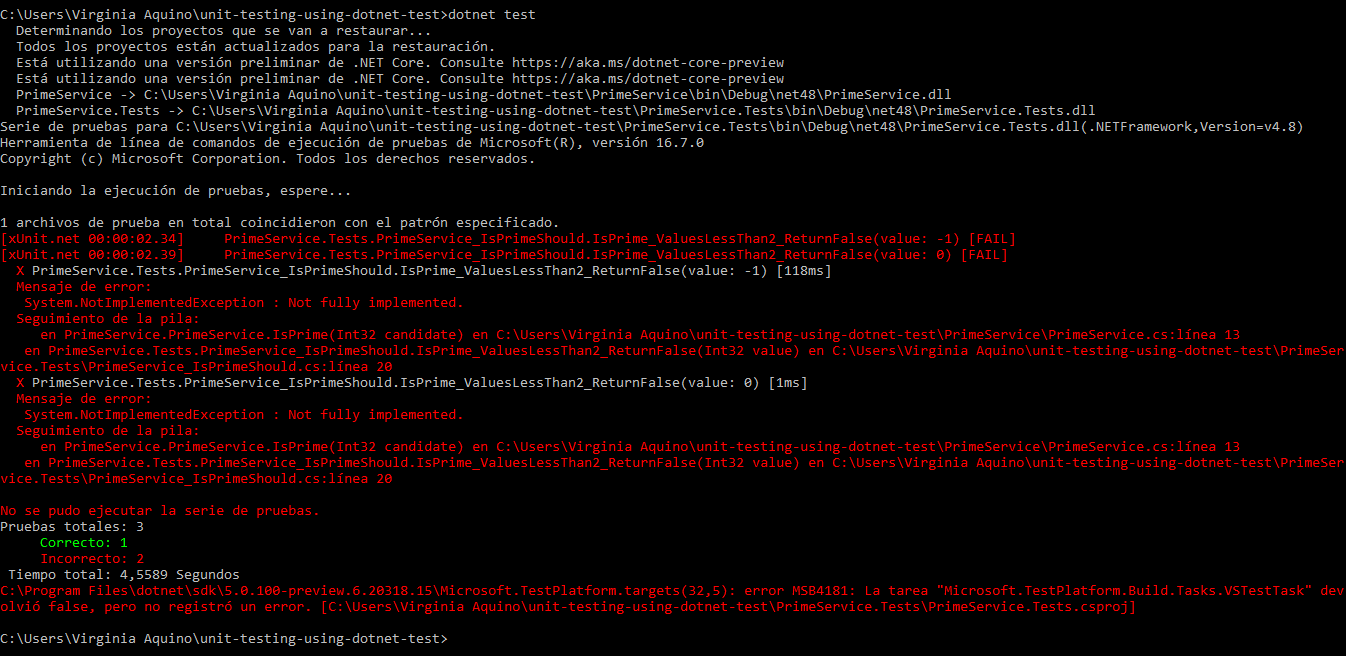
\includegraphics[width=\columnwidth]{images/resu3}\newline
\end{center} 
\item Para pasar todas las pruebas, actualice el IsPrimemétodo con el siguiente código:
\begin{center}
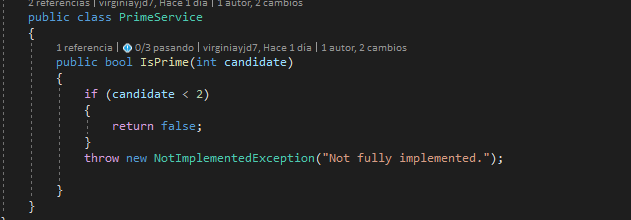
\includegraphics[width=\columnwidth]{images/lab6}\newline
\end{center} 
\item  actualice el código de destino.El IsPrime método completado no es un algoritmo eficiente para probar la primalidad.
\begin{center}
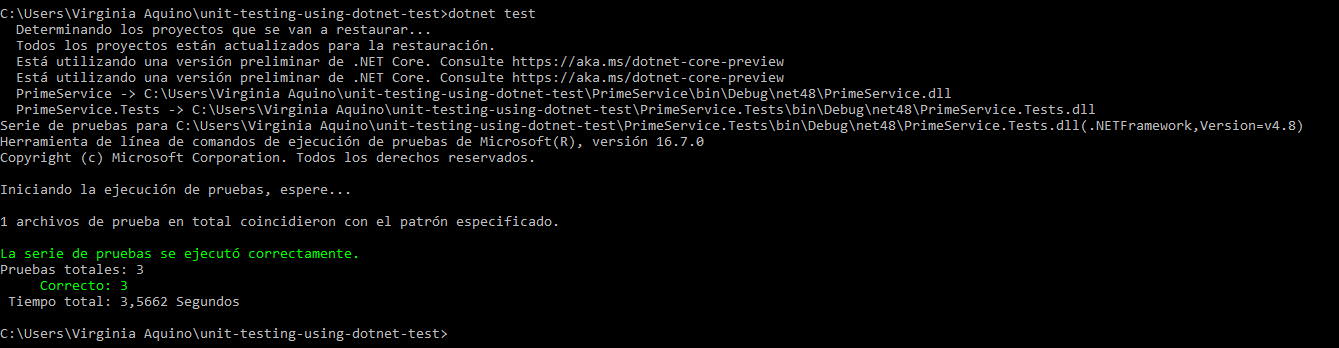
\includegraphics[width=\columnwidth]{images/final}\newline
\end{center} 
\end{itemize}


